\chapter{Anleitungen}
\label{chap:teil2_anleitungen}

Die nachfolgende Tabelle zeigt einige der wichtigsten Pakete\index{Paket}, die in der Bachelor-Thesis \LaTeX{} Vorlage verwendet werden.

\begin{table}[H]
	\centering
	\begin{tabular}{p{0.13\textwidth} p{0.75\textwidth}} \toprule
		\textbf{Paket} & \textbf{Funktion} \\ \midrule
		\texttt{cmbright}\index{cmbright} & Serifenlose Schriftart 'Computer Modern Bright' welche die Textcodierungen\index{Textcodierungen} OT1, T1 und TS1 unterst�tzt, sowie die mathematischen Zeichen wie auch die AMS Symbole \\ \midrule
		\texttt{ae} & Sorgt f�r besser aufgel�ste Schriften in PDF Dateien \\ \midrule
		\texttt{fancyhdr}\index{fancyhdr} & Einfache Anpassung der Kopf- und Fusszeilen \\ \midrule
		\texttt{graphicx}\index{graphicx} & Einbindung von Grafiken in \LaTeX{} dokumente \\ \midrule
		\texttt{booktabs}\index{booktabs} & Sch�nere Darstellung von Tabellen \\ \midrule
		\texttt{textpos}\index{textpos} & Vereinfachte absolute Positionierung von Boxen auf der Seite \\ \midrule
		\texttt{hyperref}\index{hyperref} & Paket zum Erstellen von Links in PDF Dateien \\ \midrule
		\texttt{geometry}\index{geometry} & Vereinfachte und verbesserte Anpassung des Standard-Satzspiegels \\ \midrule
		\texttt{makeidx}\index{makeidx} & Einfache Indexerstellung (siehe Kapitel \ref{sec:teil2_anleitungen_index})\\ \midrule
		\texttt{glossaries}\index{glossaries} & Erstellen von Glossaren (siehe Kapitel \ref{sec:teil2_anleitungen_glossar}) \\ \bottomrule
	\end{tabular}
	\caption{Pakete}
	\label{tab:teil2_pakete}
\end{table}

Die Tabelle \ref{tab:teil2_pakete_new} zeigt, welche Pakete zus�tzlich dazugekommen sind.

\begin{table}[H]
	\centering
	\begin{tabularx}{\textwidth}{|r|X|}
		\hline
		\textbf{Paket} & \textbf{Funktion} \\
		\hline
		\texttt{tabularx}	\index{tabularx}	& Paket um sch�ne Tabellen darzustellen																				\\
		\texttt{pdfpages}	\index{pdfpages}	& Einbinden von pdf-Dateien																										\\
		\texttt{nameref}	\index{nameref}		& Referenzieren per Name und nicht per Kapitelnummer (Darstellung der Links)	\\
		\texttt{dirtree}	\index{dirtree}		& Erstellen von Ordner-Datei-Strukturen																				\\
		\texttt{listings}	\index{listings}	& Paket zum darstellen von Source Code																				\\
		\hline
	\end{tabularx}
	\caption{Zus�tzliche Pakete}
	\label{tab:teil2_pakete_new}
\end{table}


\section{Stichwortverzeichnisse}
\label{sec:teil2_anleitungen_index}

\LaTeX{} ist in der Grundausstattung nicht f�hig ein \gls{StwVrz} \index{Stichwortverzeichnis} zu erstellen. Diese k�nnen in \LaTeX{} mit dem \texttt{makeidx} Paket und dem \texttt{makeindex}\index{makeindex} Programm erstellt werden. Die folgende Seite enth�lt eine ausf�hrliche Erkl�rung wie das Paket funktioniert und dessen Anwendung:

\begin{center}
	\url{http://de.wikibooks.org/wiki/LaTeX-W�rterbuch:_makeindex}
\end{center}

Grob zusammengefasst sind f�r ein Stichwortverzeichnis folgenden Punkte n�tig:

\begin{itemize}
	\item Einbinden des Paketes \texttt{makeidx}
	\item Durch den \texttt{\textbackslash makeindex} Befehl die Erstellung initialisieren
	\item Im Text laufend W�rter indexieren mit dem Befehl \texttt{\textbackslash index\{\}}
	\item Beim ersten Durchlauf der Dokumenterstellung wird das Verzeichnis erstellt und die mit \texttt{\textbackslash index\{\}} markierten Begriffe in der \texttt{.idx}-Datei gespeichert
	\item Beim zweiten Durchlauf wird die \texttt{.idx}-Datei sortiert, formatiert und als \texttt{.ind}-Datei abgespeichert, wobei \LaTeX{} nun die \texttt{.ind}-Datei in das Dokument einf�gt
\end{itemize}


\section{Glossar}
\label{sec:teil2_anleitungen_glossar}

Ein Glossar\index{Glossar} kann in \LaTeX{} ebenfalls mit dem \texttt{makeindex} Programm und dem \texttt{glossaries} Paket erstellt werden. Die folgende Auflistung zeigt das Vorgehen um ein Glossar zu erzeugen:

\begin{itemize}
	\item Einbinden des \texttt{glossaries} Pakets
	\item Falls es als sinnvoll erachtet wird, kann eine eigene Datenbank mit Glossareintr�gen erstellt werden. In dieser Vorlage wird mit einer solchen Datenbank gearbeitet, welche im Ordner \texttt{datenbanken} abgelegt ist. Eintr�ge aus der Datenbank werden nur in das Verzeichnis geschrieben, falls das Wort im Text auch wirklich vermerkt ist.
	\item Durch den \texttt{\textbackslash makeglossaries} Befehl wird die Erstellung initialisiert
	\item Neue Eintr�ge k�nnen mit dem Befehl \\ \texttt{\textbackslash newglossaryentry\{<ABK�RZUNG>\}\{name=\{<NAME>\},description=\{<BESCHRIEB>\}\}} \\ erstellt werden
	\item Im Text laufend W�rter referenzieren mit dem Befehl \texttt{\textbackslash gls\{<ABK�RZUNG>\}}
	\item �hnlich wie bei der Erstellung des Index, wird das Verzeichnis erst beim zweiten Durchlauf in das Dokument eingebunden
\end{itemize}

Damit das Ganze �berhaupt funktioniert, muss als Nachbearbeitung des Dokuments das Glossar mit \texttt{makeindex} erstellt werden. Dazu ist folgender Code in der Kommandozeile auszuf�hren:

\begin{center}
	\texttt{makeindex -s template.ist -t template.glg -o template.gls template.glo}
\end{center}

Bei den meisten \LaTeX -Editoren kann dies als Nachbearbeitungsschritt angegeben werden. Die nachfolgende Erkl�rung ist f�r das Programm TeXnicCenter. Unter dem Menupunkt \glqq Ausgabe\grqq{} -> \glqq Ausgabeprofile definieren\grqq{} (kurz: alt + F7) ist unter dem Register \glqq Nachbearbeitung\grqq{} das in Bild \ref{fig:teil2_nachbearbeitung} dargestellte Fenster zu finden. Anschliessend gilt es, einen neuen Eintrag einzuf�gen, wobei eine Anwendung wie auch ein Argument anzugeben ist. Die Anwendung ist in der MiKTeX Installation zu finden (\texttt{..\textbackslash MiKTeX X.X\textbackslash miktex\textbackslash bin\textbackslash makeindex.exe}). Als Argument ist die folgende Zeile eizutragen:

\begin{center}
	\texttt{-s \string"\%tm.ist\string" -t \string"\%tm.glg\string" -o \string"\%tm.gls\string" \string"\%tm.glo\string" }
\end{center}

\begin{figure}[H]
	\centering
	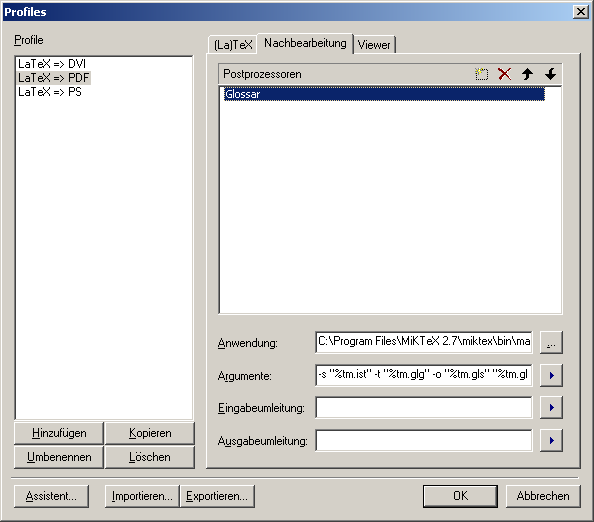
\includegraphics[scale=0.7]{bilder/profiles_glossar.png}
	\caption{Nachbearbeitung}
	\label{fig:teil2_nachbearbeitung}
\end{figure}


\section{Bibliographie}
\label{sec:teil2_anleitungen_bibliographie}

Zur Erstellung einer Bibliographie\index{Bibliographie} wird auf \gls{BibTeX} zur�ckgegriffen. Im Ordner \texttt{datenbanken} befindet sich eine \texttt{.bib}-Datei mit diversen Datenbankeintr�gen. Wie diese Eintr�ge zu erstellen sind, kann aus diversen Quellen im Internet oder in B�chern entnommen werden. Die Eintr�ge in der Datenbank werden nur dann in das Verzeichnis des Dokuments geschrieben, wenn die Quelle auch wirklich im Text zitiert wurde.

Unter den folgenden Adressen sind weitere Erl�uterungen zum Erstellen der Datenbank und deren Verwendung zu finden:
\begin{itemize}
	\item \url{http://en.wikipedia.org/wiki/BibTeX}
	\item \url{http://www.bibtex.org/de/}
\end{itemize}


